% !TEX root=frame_thesis.tex
\chapter{Methods and Model Description}

\section{Overview of the Model}
%Topic: General overview of ABM
%Main Idea: Human agents interact with local Environment
In this thesis, I present an Agent Based Model (ABM) that simulates the temporal and spatial pattens of household agents on Easter Island and their interaction with the natural environment. 
The environment is encoded on a 2D discretised map with real geographic features.
Agents rely both on a non- or slowly renewable resource, the palm trees, and a renewable resource, land for agriculture, in particular sweet potato cultivation. 
They obtain these resources by cutting trees and occupying viable sites with gardens in their near surroundings, thereby changing their local environment.
Consequently, the household's population growth or decline depends on the success of this resource allocation. 
Furthermore, resource availability determines the settlement behaviour of the agents.
The interaction with the natural environment places constraints on the settlement patterns as well as the population dynamics of the overall Easter Island society.

%Topic: Time and Update Order
The model assumes yearly updates of the variables of each household agent and the environment throughout the time period of the prehistoric Easter Island society.
The simulation starts with the arrival of the first settlers at Anakena Beach in $t_\text{arrival} = 800\, {\rm A.D.}$. 
The initial population is assumed to be 40 individuals spread on 2 households (40 in \citet{Good2006} and 20 to 100 in \citet{Brander1998}, 50 in \citet{Brandt2015}).
In each time step, $\Delta t=1\,{\rm yr}$, all agents are updated sequentially in a random order. 
A single update comprises the interaction between the agent and the environment, consequent changes of the variables, adjustment of the agent specific parameters, population growth/decline and potential re-settlement.
New household agents can appear throughout the simulation following reproduction and splitting of existing agents. 
The simulation ends in $1800\, {\rm A.D.}$ with the arrival of European voyages marking the end of the isolated status of the Easter Island society.%, since this presumably had a large impact on the society, e.g.\ through the introduction of diseases wiping out a large fraction of the Easter Island population in the 19th century.% \todo{cite Bahn2017}.

%Topic: I will describe the Model
In Section \ref{sec:CreateMap}, I describe the generation of the 2D discretised map comprising the environment of Easter Island. In Section \ref{sec:AgentUpdate}, I then focus on the household agents and the update of a single agent.
This update is separated into several modules: Calculating of the agents' resource requirements, cutting trees, farming, increasing/decreasing population of the agent, and potentially moving the settlement.
Figure \ref{fig:SketchABM} summarises all environmental variables, the agent variables, and their dependencies.


\begin{figure}[H]
	\centering
	%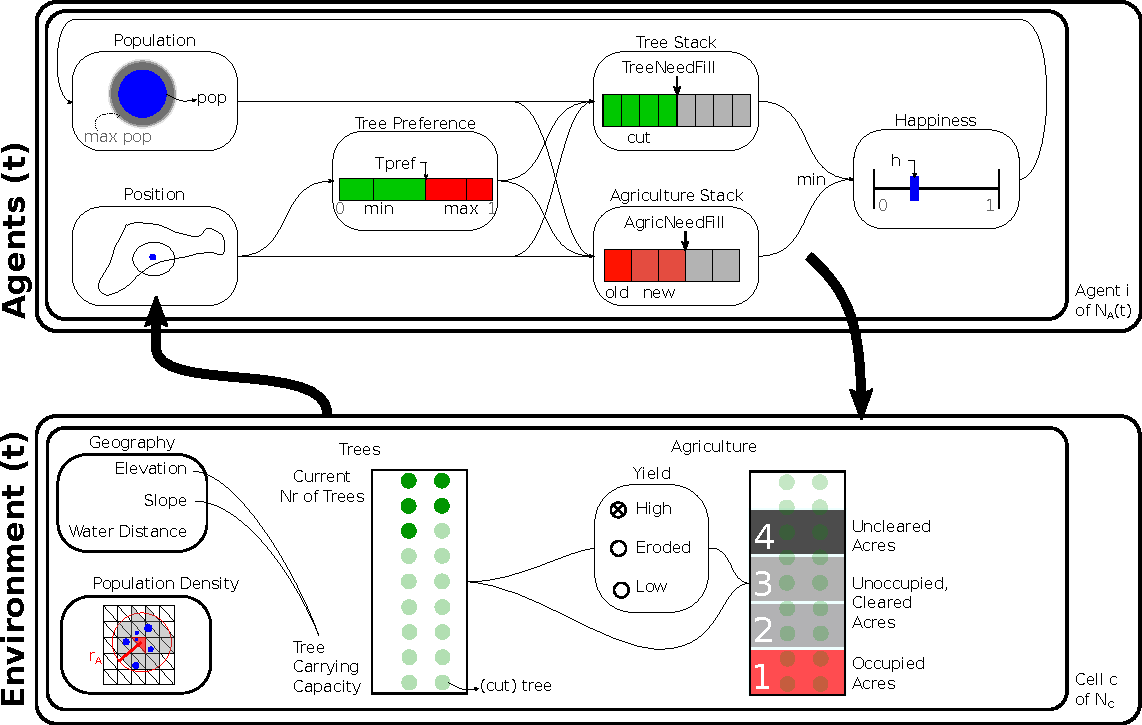
\includegraphics[width=1\textwidth]{images/SketchABM/SketchABM.pdf}
	\caption{
		A sketch of the ABM presented here and described in detail in Chapter \ref{chapter:Methods}.
		The environment consists of $N_\text{c}$ discretised cells, $c$, with certain geographic properties: Terrain elevation $el(c)$, slope $sl(c)$, area, $A(c)$, %population density $\frac{pop(C_\text{F}(t)}{r_\text{F}^2\pi}$) (within cells in a circle with radius $r_F$, $C_F(c)$) 
		and the two `resource stock' variables.
		The first stock variable of a cell is the number of trees $T(c,t)$.
		The maximum stock is the cell's carrying capacity and initial state, $T(c,t=0)$, which depends on the terrain elevation $el(c)$ and $sl(c)$. 
		The second stock of a cell is the number of arable (i.e.\ Productivity index $F_{\rm PI}(c,t)>0$) sites, $F_\text{arable}(c,t)$, with a basic unit of $1\, {\rm acre}$, in combination with the number of occupied sites, $F_\text{occ}(c,t)$ in acres.
		Agents are households with a population size $pop_\text{i}(t)$, a settlement location $(x_\text{i},\, y_\text{i})$ (corresponding cell $c_\text{i}(t)$), a tree preference $T_\text{pref, \, i}(t)$ depending on the tree stock of the local environment, and corresponding requirements for tree cutting, $T_\text{req, \, i}(t)$ and farming, $F_\text{requ, \, i}(t)$, depending on the tree preference and global constants, baseline tree and farming requirements per person, $T_{requ, \, pP}$ and  $F_\text{requ, \, pP}$.
		The success of meeting these requirements depends on the resource stocks of cells in radii $r_T$ for tree harvest and $r_F$ for farming. 
		The resulting current and smoothed happiness indices, $h_\text{i}(t)$ and $H_\text{i}(t)$ then determine the agent's population dynamics.
		Finally, for insufficiently small smoothed happiness (i.e.\ when the agent's net population size decreases) the settlement is moved to a new location in a complex, semi-rational, individual decision making process through evaluating sites according to multiple environmental factors.
	}
	\label{fig:SketchABM}
\end{figure}


\section{Creating a 2D discretised Map of Easter Island}

First, a discretised map is created dividing the island into a number of small 2D triangular cells with certain geographical features via a triangulation of a rectangular grid of points.
I use a 2D equidistant grid ranging from ($-27.2050^\circ N$, \, $-109.4650^\circ E$) to ($-27.0437^\circ N$, \, $-109.2227^\circ E$) and a resolution of \todo{$\delta = points/km$}(i.e.\ $100$ points in $x$- (East) and $50$ points in $y$-direction (North)). 
In principle, the map can be created with any arbitrary resolution, constrained only by the resolution of the underlying geographical data. 
Also other grid types, e.g.\ one with higher resolution in a specific region of interest, are completely compatible with the model. 
While a higher resolution results in a more detailed and less discretisation error, computation time of the presented model scales highly non-linearly (see Section \TODO).
Hence, a trade-off has to be found between detail or accuracy and computation time.
Given this grid, I use \citet{matplotlib}\TODO's Delaunay triangulation tool to create 2D triangular cells.
A cell's location is defined by its midpoint $\vec{c} = (c_x,\, c_y)$. 
Since all cells are Delaunay triangles, the smallest angle is maximised. 
Hence, the midpoint, $\vec{c}$, provides a reasonable representation of the cell.
%Topic: Define Easter Island
%Using geographical information, the triangles making up Easter Island are selected.
The terrain features, elevation, $el(c)$, and slope, $sl(c)$, of Easter Island are obtained from a publicly available, high resolution elevation map \citep{Jarvis2008CIGAR} via Google Earth Engine \citep{gorelick2017google} and evaluated at the midpoint $\vec{c}$.
All cells located on the ocean (i.e.\ $el(c)=0$) are masked out and discarded.
The remaining ones constitute the landmass of the discretised island. 
With the resolution given above, $N_c = 11387$ cells remain. 
The area of the discretised Easter Island is $A=\TODO$, i.e.\ only a negligible fraction off from the $163.6\, {km^2}$ in reality.
with a area of once cell of $\overline{A(c)}= todo \pm todo$ \TODO.  

There are three -- or two in periods of major droughts (see \citet{Rull2020}) -- permanent crater lakes on Easter Island, providing the major freshwater sources for the prehistoric Easter Island population, as discussed later in Section \ref{sec:Moving}.
The corresponding cells are calculated from the locations and radii of these lakes. 
This procedure gives a detailed, discretised representation via triangular cells with geographical features of Easter Island. 
 
%Archaeological records indicate that crater lakes could have dried out during major drought periods.
%In particular the drying of Rano Raraku in the East of Easter Island during the Medieval Climate Anomaly ($500-1200 \, \rm{A.D.}$) and during the Little Ice Age ($1570-1720\, \rm{A.D.}$) \citep{Rull2020} and the consequences have been a reoccuring theme of scientific debate (e.g.\ \citet{Cauwe2011}). 
%Such drought events can be simulated by removing each of the lakes for some period of time from the map.

Furthermore, all cells have constant biological features.% next to the geographic specification before. 
Each cell $c$ has a variable tree number, denoted as $T(c,t)$ (or tree density $T(c,t)/A(c)$.
At the time of the arrival of the first settlers, the islands forest system was in equilibrium (e.g.\ \citet{Brander1998}) except for possible climatic changes, which impacted tree cover change over time \citep{Rull2020}, which are not considered here. 
Therefore, the tree number on each cell before human occupation $T(c,t=t_\text{arrival})$, constitutes a carrying capacity of palm trees for this cell. 
I assume this carrying capacity to be constant throughout the simulation.
There is is still a lot of uncertainty about the total number and patterns of palm trees at the time of arrival of the first settlers. 
\citet{MiethBork2015} estimate from root casts a total of $16\cdot 10^6$ trees covering $80\%$ of the island, whereas \citet{Brandt2015} initialise the model with a conservative estimate of $8\cdot 10^6$ trees. 
Most studies assume an island wide, dense distribution of the palm trees. 
E.g.\ \citet{Bahn2017} state that soil sufficient for tree growth is present `almost everywhere on the island, apart from the steepest parts of the cliffs and the youngest lava surfaces' (i.e.\ the highest elevations of Mount Terevaka). 
However, \citet{Rull2020} also investigates the possibility of mosaic vegetation patterns with high densities of trees around the lakes and the coastal areas.
%As mentioned in the introduction \TODO, there's no comprehensive record of tree patterns. While some \todo{cite Rull?} archaeologsits state that the majority ($80\%$ of the island) was densley forrested \todo{cite}. 
The model presented here can incorporate any pattern of pre-arrival tree density. 
For the results in this thesis, I assume an equal density pattern characterised excluding those cells with very high elevation or slope ($el(c)>430\, {\rm m}$ or $sl(c)>10^\circ$ $\Rightarrow$ $T(c,t) = 0$).
%by two terrain-dependent tree density levels: (1) `normal density' for low elevation $el(c)<250\, \rm{m}$ and slope $sl(c)<5^\circ$, (2) `half density' for moderately high elevations $250\, \rm{m}el(c)<430\, \rm{m}$ (elevation of Lake Rano Aroi) and slope $5^\circ < sl(c) < 9^\circ$, and (3) `zero density' for cells above these thresholds.
In this model, a total of 
\begin{equation}
\mathbf{T}(t=t_\text{arrival}) = \sum_{c} \, T(c,t=t_\text{arrival}) =  16 \cdot 10^6
\end{equation} 
trees (iterated over all cells, denoted by the bold symbol) are distributed with uniform probability among all cells with potential tree for tree growth. 
A resulting map of pre-arrival tree numbers $T(c,t_\text{arrival})$ in cells $c$ extending on $80\%$\TODO of Easter Island is shown in Figure \ref{fig:Map_tree}.

\begin{figure}
	\centering
	%\includegraphics[width=\textiwdth]{images/CarryingCap.pdf}
	\caption{The carrying capacity density of trees in each cell}
	\label{fig:Map_tree}
\end{figure}

Through anthropogenic deforestation, the variable tree number in each cell, $T(c,t)$, is decreased over time.
The importance of this human influence in degrading the environment compared to the impact made by a quickly increasing number of Polynesian rats is a strongly debated topic (e.g.\ \citet{Bahn2017} and \citet{Hunt2007} as described in the Introduction).
However, there seems to be a consensus between both theories that rats effectively hindered tree regeneration by gnawing on the palm nuts.
In line with these arguments, forest regeneration is not possible in the standard setting of this model.
Thus, trees constitute an entirely non-renewable resource in this case. 
However, I further explore alternative experiments in which the forest can hypothetically regenerate following anthropogenic deforestation.
Each year, tree numbers in all cells regrow logistically to their (local) carrying capacity $T(c,t=t_\text{Arrival})$ if there is no farming activity on the specific cells.
The maximum growth rate of this localised logistic regeneration of the specific palm tree is believed to be rather slow and has even been made responsible for the ecological degradation of the island in earlier studies (e.g.\ \citet{Brander1998}).
\citet{Brandt2015} use a maximum tree regrowth rate between $0.02$ and $0.07 \, \rm{1/yr}$ for their model in the absence of rats.\TODO
In this model, experiments, in which localised forest regrowth is allowed, the logistic growth rate is thus 
\begin{equation}
g_{\rm T} = 0.05\, \rm{1/yr} \ .
\end{equation}
Some cells are deforested entirely in a single update step, disabling their regeneration in the model. 
However, forest regrowth is also possible in such cells with seeds being transported to the empty cell via e.g.\ wind, birds or human activity.
To incorporate this in the model, a small number of trees `pops up' ($0.5\%$ of the cell's carrying capacity) after a cell has been left barren, i.e.\ the cell is uncultivated and without trees, for $10$ consecutive years.
Then before any anthropogenic deforestation the tree number in the next year is
\begin{equation}
T(c,t+1)= \begin{cases}
T(c,t) + T(c,t) \cdot g_{\rm T} \cdot \left(1- \frac{T(c,t)}{T(c,0)}\right) \quad & \forall \ c \text{ with } \mathbf{A}_F(c,t)=0 \\
0.005 \cdot T(c,0)  & \forall  \ c \text{ with } T(c,t)=0 \text{ and}\\
& \mathbf{A}_{\rm F}(c,\hat{t})=0 \  \ \forall \  \hat{t} \in \{t-10, \ldots, t\} \\
0 & \text{ else }
\end{cases}
\end{equation}

In the following years, these trees (if not deforested) grow logistically.
The two experiments, with and without tree regrowth following anthropogenic deforestation, allow for testing of the impact of the Polynesian rats, assuming that they effectively hindered tree regeneration.

%Topic: Agriculture Yield
I assume that the Easter Island society did not rely solely on the non- or slowly renewable natural resource tree, but also cultivated renewable crops, in particular sweet potato as the dominant staple food source \citep{Louwagie2006}.
As described in the Introduction, Easter Island's suitability for farming, especially w.r.t.\ climate and soil, has been subject to excessive debate.
While the total potential of agricultural productivity remains uncertain, several studies identified arable sites and make a distinction between viable and non-viable land by using data on rain, climate, temperature, elevation and soil quality in agricultural models (e.g.\ \citet{Louwagie2006} and \citet{Puleston2017}).

%While the total potential of agriultural productivity remains uncertain, researchers identified viable sites and can distinguish between highly or less suitable land by using data on rain, climate, temperature, elevation and soil quality in agricultural models.
In a combined data analysis and agricultural modelling study, \citet{Puleston2017} (Figure 4) indicate sites that meet a climatic and soil quality criterion for being viable for sweet potato cultivation.
These areas are located mainly along the South, North East and West coast. 
Additionally, \citet{Puleston2017} indicate upland areas, which did not meet the viability criterion, but were nevertheless covered by patchy garden structures used by the Rapa Nui.
These added only a small fraction to the total farmed land, though.
Throughout this study, I call the corresponding cells of the discretised Easter Island map located in the viable region `well-suited' and those located in the region identified by \citet{Puleston2017} as unsuitable but nevertheless cultivated `poorly suited'.

\citet{Louwagie2006} also derives a criterion for successful cultivation of several crops based on climate and soil property measurements at several sites on the island. 
One of the studied sites (Vaitea), which coincides with the poorly suited region in \citet{Puleston2017} (compare Figure 1 of \citet{Louwagie2006} with Figure 4 of \citet{Puleston2017}), was found not suitable for farming due to insufficient nutrition availability (with a relative yield of $0-20\%$ compared to an optimal site) despite archaeological evidence of gardens in this area.
To enhance yields, the islanders used techniques like labour intensive, large-scale lithic mulching, which mainly increased moisture availability, and efficient crop management, e.g.\ plant spacing and frequent fallowing \citep{Louwagie2006}.
The per area productivity, however, remains low even with these techniques in place with nutritient availability being the main constraint.
%This non-suitable site coincides with the upland poorly suited area defined by \citet{Puleston2017} . 
The other sites in \citet{Louwagie2006} located at the foots of smaller craters along the arable coasts were classified as mostly `marginally to moderately suitable' for sweet potato cultivation for most climatic conditions with some locations showind `high suitability' especially in wet years. 
These sites are mainly located in the well-suited or poorly suited regions of the map in \citet{Pulestion2017}.
%Again, through land management and labour intensive lithic mulching these yields were enhanced, however the main constraint, nutrient availability, probably limited the success of such efforts. 
%{mention that lithic mulching mainly for water availabiliyt, but main limitation remains nutrient lack!!}

All in all, one can conclude that the expected yield of sweet potato farming strongly depends on the specific location and its climatic conditions and soil quality.
This spatial variation alone would require a complex model as well as more field research.
In this model, I build on the works by \citep{Puleston2017} and \citet{Louwagie2006}.
I use the map of well-suited and poorly suited regions from \citet{Puleston2017} and transfer it to the cells of the discretised map of Easter Island.
Throughout the simulation, the agents set up a basic unit gardens of size $1\, {\rm acre}$ on arable cells\footnote{Hence, they do not use the full area of a cell but only the number of acres that fit into the cell.}.
These acres are denoted as sites in this thesis. 
A cell has 
\begin{equation}
A_{\rm acres}(c) = \text{Rounded Down }(A(c)[\text{acres}])
\end{equation}
number of acres, which can be turned into gardens and farmed.
Following roughly the classification by \citet{Louwagie2006}, I assign Farming Productivity Indices, $F_\text{PI}(c)$, to each cell and its according sites:
\begin{eqnarray*}
F_\text{PI}|_\text{well} = 80\% & \text{ for well-suited (optimal to moderate)}\\
F_\text{PI}|_\text{poor} = 10\%  & \text{ for poorly suited (not suitable)}\\
F_\text{PI}|_\text{non-viable} = 0\% & \text{ for non-viable sites}
\end{eqnarray*}
The absolute productivity of acres of arable land in units of people it can support is taken from calculations in \citet{Puleston2017} assuming two different Nitrogen fixation scenarios (see in detail later).

As mentioned by several authors, soil erosion through radical deforestation and heavy rainfalls also constrain the farming productivity of the island especially in the later phase (e.g.\ \citet{Brander1998}, \citet{Mieth2005}, \citet{Bahn2017}, \ldots).
As trees are removed from a region, rain can wash away nutrient-rich soil and reveal less fertile ground with reduced productivity \citet{Mieth2005}.
In the model, I assume that, as a cell is completely deforested, the consequent erosion reduces the $F_\text{PI}(c)$ for well suited cells to $F_\text{PI}|_\text{eroded}=50\%$. 
This soil degradation is reverted as soon as trees pop back up, i.e.\ if the cell has been kept barren (without farming) for the previous $10$ years.

It should be emphasized that, the agricultural potential of Easter Island and its impact on the population dynamics and especially the peak population size able to live on Easter Island remains a strong limitation in this model. %in estimating the carrying capacity.
The total resulting arable land area is \TODO $\rm{km^2}$ (i.e.\ $\TODO\%$) for well-suited sites and, additionally, $\TODO\, \rm{km^2}$ (i.e.\ $\TODO\%$) for poorly suited sites.
This is in line with several different estimates of the arable land fraction \TODO \citet{Bahn2017}???
%. TODO SOMEONE SAID THAT 50\% of the land was cultivated?
The map of Farming Productivity Indices $F_\text{PI}(c)$ of all cells on Easter Island is shown in Figure \ref{fig:Map_agric}, thus defining where agents have access to farming and how productive farming would have been in this location. 

\begin{figure}
	\centering
	%\includegraphics[width=\textwidth]{images/Map_agric}
	\caption{A map of the (sweet potato) Farming Productivity Indices, $F_\text{PI}(c)$, in each cell of the discretised map of Easter Island. The model makes use of the map of \citet{Pulestion2017} classifying arable land into viable areas (here `well-suited sites'), non-viable but nevertheless partially farmed (here `poorly suited sites'), and non-viable sites derived from an agricultural model of climate and soil quality. 
	This classification is combined with measurements of land suitability in several sites \citep{Louwagie2006} giving rise to a simple, spatially explicit map of farming potential parametrised by the Farming Productivity Index $F_\text{PI}(c)$.}
	%The Farming Productivity Indices in areas where gardening was observed but that did not meet the agricultural potential of \citet{Puleston2017}'s criterion is $10\%$ in line with the result of a model of agricultural yield from measurments in one such site by \citet{Louwagie2006}.}
	\label{fig:Map_agric}
\end{figure}


\section{Agents and Agent-Environment Interaction}\label{sec:AgentUpdate}
% Topic: Agents Households with properties
The ABM consists of agents representing households situated on the discretised map derived in the previous section.
%Agents have several constant properties: 
%A reproduction rate $rr$, a moving radius $r_M$, a resource search radius 
An agent with index $i$ has several varying properties describing its state at time $t$.
The settlement is located at 
\begin{equation}
	\vec{x}(t) = (x_i,\, y_i)(t)
\end{equation}
 on the discretised map and, hence, associated with one specific cell $c_i(t)$.
 The agent's population size, i.e.\ the number of individuals in the household, 
 \begin{equation}pop_i(t) \end{equation}
 typically ranges from $12$ (minimum $6$) to ca.\ $42$.% ranging from $6$ to $42$ .
While, all calculations and decisions on harvest and moving happen on the individual scale, macroscopic indicators, like the total population of the farmed land in a cell, can be calculated simply by iterating over all agents. 
Iterations over all agents (or cells of the map for the corresponding variables) are denoted via bold symbols in all equations in this thesis.

Agents rely on an intake of resources each year in order to sustain and potentially increase their population size.
As mentioned before, I consider two major resources, trees and sweet potato farming, accessible through interaction with the environment.
An agent $i$ can harvest resources from environmental cells whose midpoints $\vec{\tilde{c}}$ are within certain, fixed radii of the agent's location:
\begin{equation} \label{eq:Circle_T}
C_{T}(c_i(t)) = \{ \tilde{c}\ | \   | |  \vec{\tilde{c}} - \vec{x_i}(t) | |  \leq r_{T} \} 
\end{equation}
for resource tree with tree search radius $r_T =2\, {\rm km}$ and 
\begin{equation} \label{eq:Circle_F}
C_{F}(c_i(t)) = \{ \tilde{c}\ | \   | |  \vec{\tilde{c}} - \vec{x_i}(t) | |  \leq r_{F} \}
\end{equation}
for farming sites with farming radius $r_F = 1\, {\rm km}$.

An agent's required total resource uptake per year varies with the population size 
This resource uptake is split between trees and farming yield.
The shares are given by a trait parameter, the tree preference $T_\text{Pref, i}(t)$ for agent $i$ at time $t$, which reflects the agent's harvest behaviour in response to its local environment.
In the first settlement phase, the islanders mainly lived off the abundant natural resources of the island, i.e.\ birds, fish, and fruit from the trees \citet{Bahn2017}. 
Over time, the economy `switched from predominantly hunter-gatherer to a dryland farming society' \citep{Louwagie2006}.
In the model, this behavioural shift results from a decrease in the variable adaptive tree preference parameter, $T_\text{Pref i}(t)$ of each agent over time.
The idea of this trait parameter is that agent's adapt their resource requirements to changes in the local environment, in particular the deforestation. 
%It is an adaptive trait reflecting the local state of the environment around an agent, in particular the local abundance of trees. %(i.e.\ trees $T(c,t)$ of cells within $C_T(c_\text{i}(t)$).
Hence, as the island's trees are removed and more arable land is cleared freeing space for agriculture, the agent's tree preference decreases and farming activity increases, accordingly.
%This tree preference indicates the value of tree harvest over agricultural production and, hence, increases the need for one over the other in order to fill the resource requirements.
%The tree preference is high in the initial state, but decreases as trees become scarce and more land is available for cultivation of crops.
%Hence, $TPref_i(t)$ responds to some degree to the local environment of the agent.
In this model, the tree preference, $T_\text{Pref, i}(t)$, depends on the local, relative change of tree density within the tree search radius $r_T$ with respect to the initial state at $t=t_\text{arrival}$, i.e.:
\begin{equation}\label{eq:TPref}
T_\text{Pref, i}(t) = f\left( \, \frac{\sum_{\tilde{c} \in C_{T}(c_i(t)) } \, T(\tilde{c}, t)}{\sum_{\tilde{c} \in C_{T}(c_i(t))} \, T(\tilde{c}, t_\text{arrival}) } \, \right)
\end{equation}
The shape of the function indicates an indicator of the responsiveness of the economy/society to environmental change. How fast do agents adapt their harvest behaviour, when the non-renewable resource,the trees, is depleted from the initial state?  
I consider four possibilities (see also Figure \ref{fig:TPref_T}): The tree preference $T_\text{Pref, i}(t)$ decreases
\begin{itemize}
	\item linearly with the local, relative tree density decline (linear case).  
	\item delayed with the local, relative tree density decline (delayed case).
	\item quicker than the local, relative tree density decline (careful case),
	\item first delayed, and at some point quicker than the local, relative tree density decline (switched case) 
\end{itemize}
\begin{figure}
	\centering
	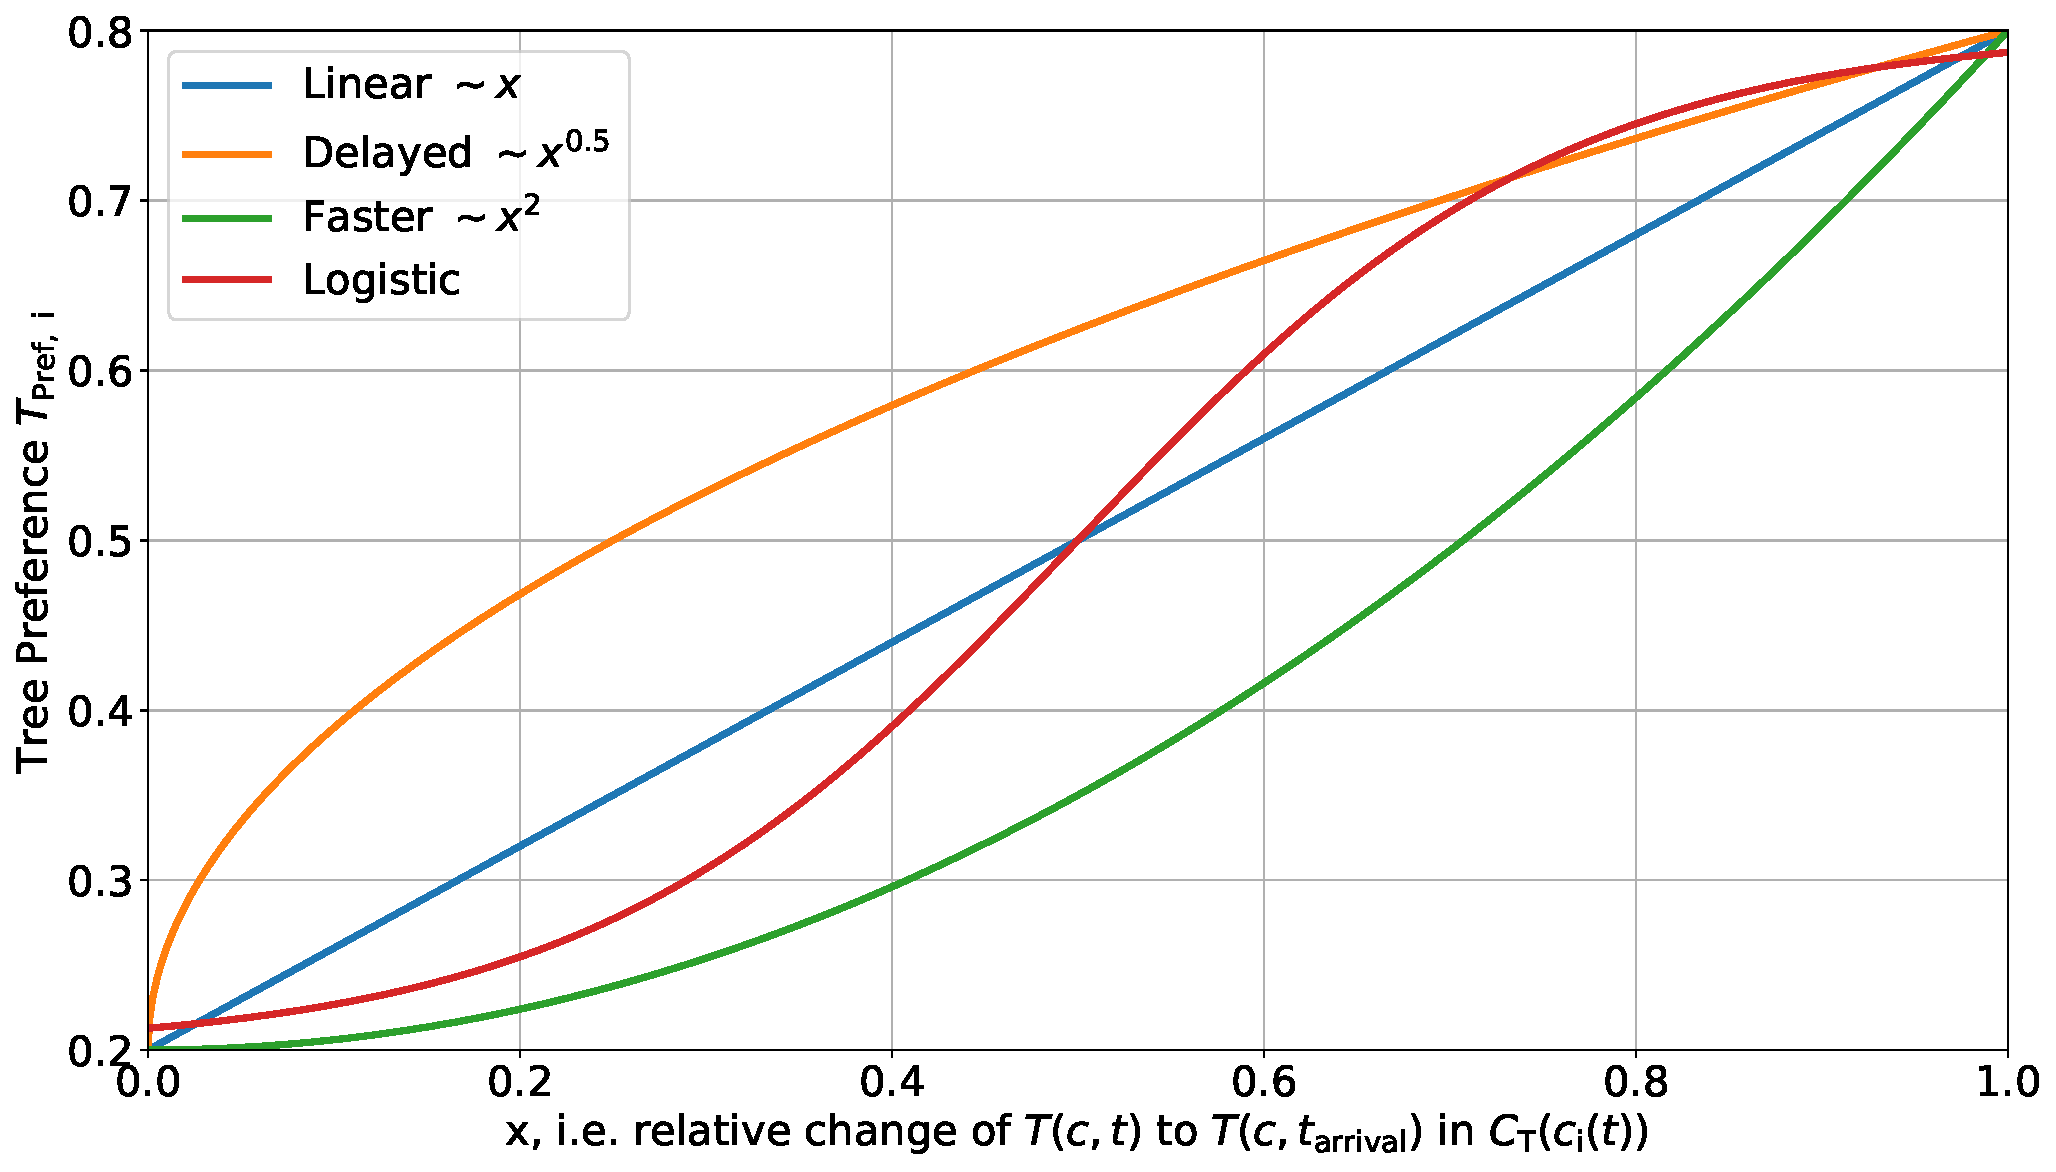
\includegraphics[width=\textwidth]{images/TPref}
	\caption{The relation of an agent's tree preference, $T_\text{Pref, i}(t)$, to relative changes in the local tree density for the four considered adaptive types with $x$ given in equation~\ref{eq:TPref}.}
	\label{fig:TPref_T}
\end{figure}
The tree preference is cut off at certain minimum and maximum thresholds, assuming an agent can not live purely off trees (and associated derivative products) and some tree cutting is required even for maximum agricultural production (e.g.\ as cooking wood or for tools). 
Here, I choose: 
\begin{equation}
T_\text{Pref, min} = 0.2 \quad \text{and} \quad T_\text{Pref, max} = 0.8
\end{equation} 
In the standard setting in this model, I use the linear relation and, hence, 
\begin{equation}
	T_\text{Pref, i}(t) =  \frac{\sum_{\tilde{c} \in C_{T}(c_i(t)) } \, T(\tilde{c}, t)}{\sum_{\tilde{c} \in C_{T}(c_i(t))} \, T(\tilde{c}, t_\text{arrival}) } \cdot (T_\text{Pref, max}-T_\text{Pref, min}) + T_\text{Pref, min}
\end{equation}
Since tree density is maximal at $t=t_\text{arrival}$, the initial agents start with maximal tree preference of $T_\text{Pref, i}(t=t_\text{arrival} = 0.8 \  \forall \ i$.


In total, the agent's resource requirements of tree harvest, $T_\text{Req, i}(t)$, and agricultural production, $F_\text{Req, i}(t)$, per year are calculated as:
\begin{equation}
T_\text{Req, i}(t) = T_\text{Pref, i}(t) \cdot pop_{\rm i}(t) \cdot T_\text{Req, pP} \, 
\end{equation}
and, similarly, 
\begin{equation}
F_\text{Req, i}(t) = (1-T_\text{Pref, i}(t)) \cdot pop_{\rm i}(t) \cdot F_\text{Req, pP}\, , 
\end{equation}
where $T_\text{Req, pP}$ is the tree requirement per year per person in absence of agriculture and $F_\text{Req, pP}$ is the required agriculture production per year in the absence of trees.
These parameters are crucial for the temporal development of the island's environment. 

The tree requirement per person (in the absence of other food sources) in principle depends on a multitude of factors, e.g.\ whether sugary sap from cut tree trunks was used as freshwater replacement as suggested by \citet{Mieth2015}.
Here, I use a constant parameter of 
\begin{equation}
T_\text{Req, pP} = 5\, \frac{\text{Trees}}{\rm person\cdot yr}
\end{equation}
(for the standard model settings) based on the maximum harvest rate used in \citet{Brandt2015}, ca.\ $3$ to $7$ trees per year\footnote{\citet{Brandt2015} use a only half of the initial trees before arrival of the first settlers, though)}. 
%In the standard run I am using $5$ Trees per Person per year. However, I vary this parameter in a sensitivity analysis (see Section \ref{sec:SensitivityAnalysis}).

The agriculture requirement per person is connected to the set up of the agricultural model resulting in productivity indices $F_\text{PI}(c)$ (Figure \ref{fig:Map_agric}).
\citet{Puleston2017} simulate the nutritional productivity of farming on `well suited' land for two different environmental scenarios for the Nitrogen fixation in the soil, i.e.\ the rate at which Nitrogen is renewed, representing a major uncertainty in their model.
This can be converted into the minimum land required to sustain one person using the nutrition content of sweet potato ($1\, \rm{t/yr}$ roughly sustains $1$ individual in the absence of other food sources): 
\begin{equation}
F_\text{Req, i}(t) = \begin{cases}
	0.5 \, {\rm \frac{acre}{person} } & \text{ for high N fixation} \\
	1.7 \, {\rm \frac{acre}{person} } & \text{ for low N fixation} \\
 \end{cases}
\end{equation}
%For $AReq\_pP$, I am using the estimates by \citet{Puleston2017}. In their agricultural model, they identify the Nitrogen fixation as a major uncertainty in the evaluation of potential agricultural yields. 
%With two different assumptions of Nitrogen fixation in the soil (high and low), \citet{Puleston2017} model the sweet potato harvest on a high quality agriculture site and combine it with the nutritional need of an individual person.
I do not consider fallowing of arable land in the model to increase its productivity, as this in general reduces the yield per total area needed for each individual (see Table 1 in \citet{Puleston2017}).
In fact, the only constrain for farming is availability of arable land in this model, not workforce or social structure (as in \citet{Puleston2017})
%One can then calculate that for high N-fixation for one person (in the abesence of other food) needs $0.5\, \rm{acres}$ of high quality agricultural productivity of sweet potato cultivation.
%In the case of low N-fixation this increase to $1.7\, \rm{acres}$ per Person. 
%Here, I am using both values in order to test the different scenarios.
The resource requirements for trees given in absolute numbers and agricultural production given in acres of well-suited quality agriculture sites are thus agent-specific features updated each year, which can be adjusted through the global parameters $T_\text{Req, pP}$ and $F_\text{Req, pP}$.

% Topic: Fishing Agents constrained by a tabu 
The model, furthermore, allows for open sea fishing as a replacement for farming for some agents living near the Anakena coast.
%Instead of filling the agricultural requirement by cultivating land with crops, these deep-sea fishing household agents obtain their nutrition from the sea in the model. 
%For such fishing agents, the agriculture and tree requirement are calculated in the same way. However 
Instead of occupying arable land units and farming, these fishers gain sufficient agricultural resources by going out to sea.
In the initial phase of Easter Island settlement, excavations prove that shellfish, fish and even porpoise were a major part of the diet at the time \citep{Bahn2017}.
However, over time, these natural resources became increasingly scarce and many species even went extinct due to human predation, with open ocean fish vanishing from the diet eventually \citep{Diamond2011}.
As a resource management institution the Easter Island society had taboos on the harvest of natural resources \citep{Good2006}. 
Fishing was mainly restricted to members of a specific chiefdom (`Miru') living at Anakena Beach \citep{Bahn2017} who would then presumably trade with others.
%According to \citet{Bahn2017} or \citet{Diamond2011}, sea fish vanished from the Easter Island typical diet by \TODO.
Hence, in the model, every agent living within farming radius, $r_F$, distance of Anakena Beach (in cell $c_{\rm Anakena}$) automatically becomes a fishing agent.
\begin{equation}
 	c_{\rm i} \in C_{\rm F}(c_{\rm Anakena}) \quad \Rightarrow \text{Agent i  fishes}
\end{equation}
\TODO TABOO? Needed??
%At time $t_\text{taboo fishing}=$\TODO a taboo is put in place externally.
%Consequently no new fishing agent's are accepted .
% letting only \TODO those agents already pursuing fishing to continue but allowing no further agents to enter this resource stock. 
While I assume that fish supply in the sea is unlimited for those living at Anakena Beach, another constraint for the agents is the requirement for trees.
For fishers this would probably be quite extensive in order to building the canoes or provide firewood. 
Hence, the fisher's minimum tree preference is increased to
\begin{equation}
T_\text{Pref, min}|_\text{fisher} = 0.5
\end{equation} 
rather than $T_\text{Pref, min} = 0.2$ for farming agents.
While fishing agents near Anakena Beach do not have any agricultural requirements due to their access to an unlimited resource stock from the sea, the correspondingly higher requirement for trees and an externally introduced restriction limit the total amount of this resource extraction.

\subsection{Agent-Environment Interaction -- Tree and Agriculture Harvest}\label{sec:Harvest}
%\begin{itemize}
%	\item Tree Harvest
%	\item Agriculture harvest
%	\item How many trees to burn
%	\item Fishing 
%\end{itemize}

%. TODO: CHANGE T REQ TO R_T and R_F 
% Topic: Tree Harvest
\paragraph{Farming}
After determining the required amount of trees, $T_\text{Req, i}(t)$, and agricultural production, $F_\text{Req, i}(t)$, as described in the previous section, an agent tries to fill these.

An agent occupies arable land unit sites, $A_\text{F, i}(t)$, with a fixed area of $1\, \text{acre}$ associated to one cell on the discretised map and obtains a yearly harvest of
\begin{equation}\label{AProd}
F_\text{i}(t) = \sum_{a \, \in \, A_\text{F, i}(t)} \, F_{PI}(c(a))\ ,
\end{equation}
where $a$ denotes a farmed acre and $c(a)$ is the corresponding cell of this acre.
Note, for fishers $F_\text{i}(t) = F_\text{Req, i}(t)$ without farming.
Agents keep all their currently occupied sites $A_\text{F, i}(t)$ until the next year.%, i.e.\ $acres_i(t+1) = acres_i(t) + new\_acres(t+1)$.
If the requirement for farming,  $F_\text{Req, i}(t)$, in the next year ($t$\ra $t+1$) increases, agent $i$ might need to acquire more arable land.
New sites are, thus, only occupied in the model if either an agent's population grows, its tree preference decreases or the soil quality of an agent's occupied sites degrades due to erosion, i.e., in summary, if an agent's farming requirement exceeds the previous agricultural production, i.e.\ if 
\begin{equation}
	F_\text{i}(t-1) < A_\text{F, i}(t) \ .
\end{equation}
Then the agent occupies more sites extending $A_\text{F, i}(t)$ and thus increasing the produce $F_\text{i}(t)$.
%By occupying and farming a basic units of $1\, \text{acre}$ of arable land an agent increases the harvest $F_\text{i}(t)$ (in units of ${\rmacre}$)until it exceeds the required $F_\text{Req, i}(t)$.
%The list of occupied sites by agent $i$ is denoted as $A_\text{F, i}(t)$, in which each acre is associated with one cell ($c(a)$ for $a \in A_\text{F, i}(t)$) and the resulting harvest obtained from these is:
%\begin{equation}\label{AProd}
%F_\text{i}(t) = \sum_{a \, \in \, A_\text{F, i}(t)} \, F_{PI}(c(a))
%\end{equation}
%The agent increases $AProd_i(t)$ by occupying more sites and adding them to $A_\text{F, i}(t)$ until there are no further sites available or the requirement $AProd_i(t) \geq ARequ_i(t)$ is fulfilled.

In the search for new farming sites, an agent first considers only sites in well-suited cells, i.e.\ $c \in C_\text{F}(c_\text{i}(t))$ with $F_\text{PI}(c)=1$, in order to maximise efficiency.
An acre in an arable cell can only be occupied (or added to $A_\text{F, i}(t)$) if at least this one acre is cleared off trees and not occupied. 
Assuming that the trees are evenly distributed on the cell's area, the condition can be calculated as 
\begin{eqnarray}
%& \text{Treeless Area\,[acre]} - \text{Occupied Acres\,[acre]}  & \geq 1  \\
%\Leftrightarrow & 
\left( 1 - \frac{T(c,t)}{T(c,0)} \right) \cdot A(c) - \mathbf{A}_\text{F}(c, t) & \geq   1
\label{eq:BurningCond}
\end{eqnarray}
where the first term is the treeless area in ${\rm acres}$ and the second term, $\mathbf{A}_\text{F}(c, t)$ is the number of farmed acres (by any agent) in cell $c$.

If there are no well-suited sites left that fulfil this condition, the agent uses the slash and burn method to reduce the number of trees $T(c,t)$ of an available well-suited cell $c$.
The agent starts with the cell, that requires the least amount of trees removed for the condition to hold.
But it continues until the farming requirement is exceeded or all well-suited acres are occupied.
The use of fires to clear space is supported by the extensive charcoal record starting with the period of intensified agriculture \citep{Mieth2015}. 
Here, I assume that if space is required for farming trees were burned directly and independently of the continuous tree harvest .
Of course, one could also use these trees first and (e.g.\ for extracting the sugary sap) then burn the remaining material to clear the land for next year as indicated by \citet{Mieth2015}, but this would require agents that plan ahead.
%felled and used (e.g.\ for extraction of the sugar sap) before burning and consequent agricultural use of the land \citep{Mieth2015} or slash and burn method was used directly to clear space as necessary next to tree harvest %(e.g.\ indicated by \citet{Bahn2017}). % Bahn: ``fires directly accompanied by agriculture''
If, all well-suited sites within $C_F(c_i(t))$ are occupied, but the agent's agricultural production does not yet meet the farming requirement ($F_\text{i}(t)<A_\text{Req, i}(t)$, the agent also occupies eroded and then  poorly suited cells in the same procedure.

\TODO

\paragraph{Tree Harvest}
After filling the farming requirement, the agent then cuts trees according to their tree requirement $T_\text{Req, i}(t)$.
An agent $i$ selects random cells $c\in C_T(c_i(t))$ with uniform probabilities and successively removes trees from these cells until the number of cut trees, $T_\text{i}(t)$ matches the requirement $T_\text{Req, i}(t)$ or no further trees area present. 
%An agent $i$ selects random cells $c\in C_T(c_i(t))$ with probabilities proportional to the tree number $T(c,t)$ on them. \TODO?!?
%Then, the agent removes one tree successively from these cells and adds these to $TCut_i(t)$.
%This is done successively until its tree requirement is fulfilled, i.e.\ $TCut_i(t)=TRequ_i(t)$, or there are no trees left in cells within the $r_T$ distance of the agent.
Unlike farming, where occupied sites are kept and re-used (with the same productivity index) in the next update, the agent needs to find new trees every year,.% i.e.\ $TCut_i(t)$ is starts at $0$ each year.
Therefore, if tree regrowth is disabled, this tree harvest represents a non-renewable resource dependency of the Easter Island society.
While the agent's adapt their harvest behaviour via the tree preference, a minimum amount of trees is always required and, hence, there's no equilibrium state without tree regrowth.

Figure \TODO \ref{fig:treeburning} shows an example sketch of potential procedure of deforestation and consequent replacement by agriculture in an example cell. 

\begin{figure}
	\centering
	%\includegraphics[width=\textwidth]{images/sketchDeforestation.png}
	\caption{Sketch of deforestation procedure in an example cell $c$ (box). 
		In the beginning the cell has 17 of its initial 20 trees still standing. 
		The area of cell $c$ is $3.2\, \rm{acres}$. 
		Agent $a$ removes 5 trees from cell $c$ (among others potentially) to fulfil its tree requirement. An agent $b$ consequently occupies the now free space on cell $c$ for agricultural production. 
		Next, an agent $c$, needs to occupy more sites to fill its agricultural requirement as well and cannot find any other unoccupied acre in $C_A(c_c)$ despite the ones in cell $c$. 
		However the agent needs to burn $5$ trees before being able to occupy the second acre on this cell.}
	\label{fig:treeburning}
\end{figure}

\paragraph{Happiness}
An agent $i$'s happiness $h_\text{i}(t)$ after the harvest depends on the ratio between the $T_\text{i}(t)$ cut trees and $F_\text{i}(t)$ agricultural produce in comparison to the requirements determined beforehand.
%Assuming that both requirements determine  the tree requirement and the agriculture requirement is equally important to the agent, the happiness is simply the minimum of the fraction of requirements that could be filled:
By assuming that both resources are equally indispensable, the happiness is equal to the smaller of the two fractions:
\begin{equation} 
h_\text{i}(t) = min \left( \frac{T_\text{i}(t)}{T_\text{Req, i}(t)}, \, \frac{F_\text{i}(t)}{F_\text{Req, i}(t)} \right)
\label{eq:h_i}
\end{equation}
If both requirements are filled for agent $i$, the happiness is maximised $h_\text{i}(t)=1$.
However, if either $T_\text{i}(t)=0$ or $F_\text{i}(t)=0$, $h_\text{i}(t)=0$ follows regardless of the success in harvesting the other resource.

%Following the harvest action, the population size of an agent is adapted and 
%the agent's population dynamics responds and the agent might decide to re-locate the settlement.
Since households have some resilience to a decline in harvest success (e.g.\ by storing food over more successful years), a memory happiness $H_\text{i}(t)$ is calculated in each year:
\begin{equation}
H_\text{i}(t) = \begin{cases} 
				h_\text{i}(t) & \text{ if } h_\text{i}(t)\geq h_\text{i}(t-1) \\
				\frac{h_\text{i}(t) + h_\text{i}(t-1)}{2} & \text{ if } h_\text{i}(t)<h_\text{i}(t-1) 
		\end{cases}
\end{equation}
If an agent's resource availability decreases, its memory happiness decreases monotonically.
If e.g.\ all trees were to suddenly vanish within a year, an agent would have two years before its memory happiness bottoms at $H_\text{i}(t) = 0$.
In the following section, I describe the possible responses of agent $i$ depending on the memory happiness $H_\text{i}(t)$, as an indicator for successful resource acquisition.




\section{Agent's reaction to the harvest}\label{sec:Reaction} 
\subsection{Population Dynamics}

%The population of an agent is assumed to b
Following farming and tree cutting actions, the agent's population size is adapted. 
The net (positive or negative) growth rate of the agent's population at a specific time depends only on the smoothed happiness. 
\begin{equation}\label{eq:popgrowthcontinuos}
pop_{\rm i}(t+1) = g(H_{\rm i}(t)) \cdot pop_{\rm i}(t)
\end{equation}
In fact, instead of assuming continuous growth or decline according to this growth rate, $g(H_{\rm i}(t))$, the population dynamics is implemented as discrete, stochastic process.
Each individual member of the agent has a $1-g(H)$ probability to die, if $g(H)<1$, or a $g(H)-1$ chance to reproduce (i.e.\ adding one individual to the household/agent), if $g(H)>1$.
The population size stays constant at $g(H)=1$. 
This results in a growth/decline of the population where each agent's trajectory is a single realisation of the stochastic process which on average matches the continuous growth in equation~\ref{eq:popgrowthcontinuos} (compare e.g.\ with \cite{Bungartz2013}).
Figure \ref{fig:app:PopulationGrowth} \TODO in the appendix shows a few different realisations of such a growth scenario with constant growth rate $g=1.007$ (i.e.\ $H=1$) in comparison with the continuous growth.


The reproduction rate of the Easter Island population in the case of unlimited food supply, i.e.\ especially in the initial phase, is widely discussed in the literature.
Parameters used range from $0.7\%$ per year \citep{Bahn2017} or `always below $1\%$' \citep{Brander1998} to exceeding $3\%$ \citep{Hunt2006} for short periods of time or $2.3-4.5\%$ \citep{Brandt2015}.
It is clear that depending on the proposed chronology, researchers have to make very contrary assumptions on the population growth in order to fit the few undisputed facts about population dynamics on Easter Island. 
If an arrival around $1200\, \text{A.D.}$ is assumed (as in \citet{Hunt2007} or \citet{Brandt2015}), assuming a large population growth is unavoidable. 
There is no way, that only a few hundred inhabitants in the 14th and 15th century could have caused a massive alteration of the island's environment and created several hundred Moai statues.
On the other hand, many studies propose arrival dates around $800\, \text{A.D.}$(e.g.\ \citet{Bahn2017}) with older studies assuming settlements as early as $400\, \text{A.D.}$ (\citet{Good2006} and \citet{Brander1998}).
Archaeological data, e.g.\ charcoal evidence, however, suggests a period of intensification of human activity starting after $1200\, \text{A.D.}$ (e.g.\ \citet{Bahn2017}) and \citet{Hunt2006}).
Hence, these studies assume a slow but continued population growth starting with the `early' arrival.% way before $1000\, {\rm A.D.}$.% up to a peak population in $1300-1700\, \text{A.D.}$.
%, one has more freedom in choosing the initial growth rate.
%especially considering that there might have been several phases of population declines as proposed in \citet{\TODO Bahn2017}. 
%One could imagine that after initial fast growth of the population after an early arrival, through fertility control a steady population size was reached below Easter Island's resource carrying capacity. 
%Archaeological and charcoal data, however, suggest an intensification of human activity (and its impacts on the environment) only at around 1200 \citet{Hunt2007} and very little environmental impact before that.
%Most researchers rather assume a slow but continued population growth from an early arrival to a peak population around 1300-1700 (e.g.\ \citet{Brander1998}, \citet{Bahn2017})
Following \citet{Bahn2017}, I choose an early arrival date here ($t_\text{arrival}=800\, A.D.$) and a slow growth rate in the case of unlimited food supply and, therefore, happy agents: 
\begin{equation}
	g(H_\text{i}(t)=1) = 1.007
\end{equation}

The specific dependency of the population growth/decline with limited food resources is a further uncertainty.
\citet{Lee2008} have constructed a food-limited dempgraphy model which was applied for the Polynesian context \citet{Puleston2008} and extended and to Easter Island society and agricultural constraints in \citet{Puleston2017}. 
Here I take a use a strongly simplified version of this model to parametrise the impact of non-optimal harvests on the population dynamics. 
The model calculates age-dependent survival and fertility rates, which are both S-shaped curves w.r.t.\ the food availability (i.e.\ high in the case of large food availability and low in the case of scarce food availability).
Since, I do not consider (age-stratified) structures below the agent/household level, I simply assume a growth rate with the same shape as the survival and fertility rates.
\begin{equation}
g(H_\text{i}(t)) \sim CDF(\Gamma_\text{Dist}(shape, scale=0.1))
\end{equation}
where $CDF(\Gamma_\text{Dist})$ is the cumulative density function of the Gamma distribution with scale set as in \citet{Lee2008}.
I then tune the shape parameter of this function to obtain \citet{Puleston2017}'s (supplementary material)  equilibrium point $g(H_\text{i}(t) =H_\text{equ})=1$, at which the population size remains constant:
\begin{equation}
H_\text{equ}=0.6883 \quad \text{with } g(H_\text{i}(t) = H_\text{equ})=1  
\end{equation} 
In order to test sensitivity of this parametrisation, I also investigate a higher shape parameter $shape=3$\TODO, which leads to a less resilient population size as resource scarcity sets in.
In this alternative, less resilient scenario, the growth rate declines faster with food scarcity (and thus happiness $H_\text{i}(t)<1$) and $H_\text{equ, 2}=0.84$ with $g(H_\text{i}(t)=H_\text{equ, 2})=1$
The amplitude of the resulting function (for both scenarios) is scaled to give the chosen reproduction rate under unconstrained food supply from last paragraph 
$g(H_\text{i}(t)=1)=1.007$.
Figure \ref{fig:growthrate} shows the resulting two regimes of population growth (for $H_\text{i}(t)>H_\text{equ}$, with a maximum of $g(H_\text{i}(t)=1)=1.007$) and decline (for $H_\text{i}(t)<H_\text{equ}$) (standard setting in blue and less resilient setting in red).
\begin{figure}
	\centering
	%\includegraphics[width=\textwidth]{images/reproductionrate}
	\caption{}
	\label{fig:growthrate}
\end{figure}
%There are two regimes of population dynamics: a population growth for $H_\text{i}(t)>H_\text{equ}$ with maximum $g(H=1)=1.007$, and a decline for 
%At $H=1$, the households population grows with rate $1.007$, as tree or agricultural land availability decreases, the agent's smoothed happiness decreases and so does the growth rate. If $H<0.6883$, the population size decreases.

If the household size $pop_i$ of an agent $i$ falls below a certain threshold 
$pop\_min = 6$, the agent $i$ disappears and the remaining individuals are adopted by other households chosen randomly within a the moving radius distance, $r_M$ ($C_M(c_i)$ defined later).
It should be noted, that the use of the model in \citet{Pulestion2017} is strongly simplified here.
E.g.\ I am using a different notion of food/tree availability, which I express via the smoothed happiness $H_\text{i}(t)$, rather than \citet{Puleston2017}'s food ratio.
Also the distinction between survival and fertility rate especially given their age-dependency is entirely neglected.
Nevertheless, the resulting dependency of growth/decline rate on the agent's happiness (and consequently its success in resource acquisition) given in Figure \ref{fig:growthrate} seems to be a reasonable functional parametrisation. 


% Topic SPLITTING THE AGENT
If the household's population becomes too large, a subgroup emerges from it and starts a new settlement.
According to \citet{Bahn2017}, settlements found in archaeological excavations consisted of two to three dwellings, the basic domestic units (e.g.\ caves or stone houses). 
Assuming that roughly a dozen people can live in such a dwelling, which would include the larger family, a household has on average $2.5\cdot 12 = 30$ individuals.
In this model, if the population size increases to a value, such that more than three dwellings would be needed, a group of twelve individuals splits and starts a new settlement on a different location of the island. 
It is clear that the social structure of the Easter Island population is much more complex than independent, small households of a few dozen people. 
E.g.\ \citet{Cauwe2011}\TODO describes the political structure of chiefdoms, \citet{Puleston2017} consider the economic system comprising an elite and working class.
Also, there is clear evidence of exchange of goods between households, e.g.\ fish, stone tools or the Moai.
All of theses complex cooperative structures are not considered here, but each agent farms and deforests individually.
The splitting of a household occurs with a probability 
\begin{equation}
Pr_{\rm splitting} = \mathcal{N}( \mu = 3.5 \cdot 12 = 42, \sigma = 3)\ .
\end{equation}
after the previously described population size adaption.
The remaining household gives up not required farmed land.
The splitting agent, immediately moves to a new location determined by the moving process described in the following section.
Hence, an independently acting agent typically represents a household of $12$ (lower limit of $6$) to $42$ individuals.

\subsection{Moving the settlement}
% When to move
Agents move their settlement to a new location as an reaction to insufficient harvest success or after splitting from a large household to start a new settlement.
If, after the harvest, the agent's smoothed happiness is below the equilibrium point $H_\text{equ}=0.6883$ (standard setting), i.e.\ population is decreasing with $g(H_\text{i}(t))\leq 1$, the agent relocates the settlement in the hope of improving the situation.
The agent first chooses a cell among cells  within a certain radius according to probabilities indicating how highly the agent evaluates this location.
Within this new cell, the agent chooses a location with uniform probability and settles there.

% How to calculate moving radius
In the initial phase of settling, agents can choose new locations from all cells on the island.
However, if a certain population size is exceeded (here $\mathbf{pop}(t)\geq \mathbf{pop}_\text{restricted moving} = 5000 \, \rm{people}$), I externally enforce a restriction of the agents' freedom to move around freely and, therefore, only allow new settlements on a limited, less distant range of cells. 
When relocating the settlement, an agent $i$, thus, chooses from cells:
%Thus, the cells considered as potential new location for an agent $i$ are
\begin{equation}
C_{M}(c_{\rm i}, \mathbf{pop}(t)) = 
\begin{cases}
\{\tilde{c} | \ \tilde{c}\text{ on island}\} & \text{ if } \mathbf{pop}(t) <5000 \\
\{\tilde{c} | \ | | \vec{\tilde{c}} - \vec{x_{\rm i}}(t) | |
%\begin{pmatrix} \tilde{c}_x \\ \tilde{c}_y \end{pmatrix}  - \begin{pmatrix}x_i\\ y_i \end{pmatrix} 
\leq r_{\rm M} \} & \text{else} 
\end{cases}
\end{equation}
with radius $r_{\rm M} = 5\, {\rm km}$ after exceeding the population threshold.

% Topic: It's a decision making process.
%Determining the new location for an agent represents a decision-making process through evaluation of sites by the agent.
In a semi-rationale decision making process the agents decide on a new location by evaluating cells within $C_{\rm M} (c_{\rm i}, \mathbf{pop}(t))$ according to certain criteria.
The calculation of the probability to move to a specific cell bases on penalties from different categories: Distance to freshwater sources $P_W$, resource availability, $P_F$ for farming productivity and $P_T$ for trees, geographical constraints $P_G$, i.e.\ terrain elevation and slope, and population density $P_D$.
High penalties represent unfavourable conditions (in the specific category) for setting up a settlement in this location.
The choice of contributions and their functional dependency is described in the remaining section.
There is, of course, substantial freedom in determining these evaluations and the decision making process.
The framework is therefore kept flexible and other assumptions or new categories can easily be added or adjusted.

%TOPIC: LOGISITIC FUNCTIONS
Penalties for each category $P_{\rm X}$ ($X=\{\text{W,\, G,\, T,\, F, \, D}\}$) are calculated via logistic functions depending on a characteristic evaluation variable $x$.
Each penalty category is evaluated according to one characteristic variable $x$ ranging $x_{\rm min}$ to $x_{\rm max}$.
% Motivation 
I determine the shape of the functional dependence of $P_X$ on variable $x$ through thresholds $x_{\rm P0.01}$ and $x_{\rm P0.99}$ indicating the value of $x$ at which the penalty $P_{\rm X}$ is smaller than $1\%$ or larger than $99\%$, respectively, in this category $X$.
The penalty $P_{\rm X}$ in a cell $c$ with value $x(c)$ is then
\begin{eqnarray}\label{eq:P_X(c)}
	P_{\rm X}(c) & = & \frac{1}{1+\exp\left( - k_{\rm X} (x(c)-\frac{x_{\rm P0.01}+x_{\rm P0.99}}{2}) \right)} %= \\
%		& = & \begin{cases}
%	<0.01  & \text{ for }x_{\rm min}<x(c)<x_{P0.01} \\
%	\text{?}  & \text{ for } x_{P0.01}\leq x(c) \leq x_{P0.99} \\
%	>0.99  & \text{ for }x_{P0.99}<x(c) < x_{\rm max} \\	
%	\end{cases}
\end{eqnarray}
where steepness $k_{\rm X}$ is 
\begin{equation}\label{eq:k}
k_{\rm X} = \left(\frac{x_{\rm P0.99}-{x_{\rm P0.01}}}{2}\right)^{-1} \cdot \log\left(\frac{0.99}{0.01}\right) \ .
\end{equation}
to adjust the penalty at $x_{\rm P0.01}$ and $x_{\rm P0.99}$.
This function is shown in Figure \ref{fig:logF}.
\begin{figure}
	\centering
	% 
	\caption{General shape of the logistic function $f(x)$ determining the penalty given a value of the characteristic variable $x$ in any evaluation category.}
	\label{fig:logF}
\end{figure}
For each category $X$, this logistic function has the same (relative) shape between $x_{\rm P0.01}$ and $x_{\rm P0.99}$ given by $k$. 
Hence, by choosing $x_{\rm P0.01}$ and $x_{\rm P0.99}$, the sensitivity of penalty $P_X$ to differences in variable $x$ is chosen. 
If $x_{\rm P0.01}$ and $x_{\rm P0.99}$ are close together, the function converges to a sigmoid function. 
If they are far apart, the function resembles a more linear increase of penalty $P_X$ with $x$.
For $x=\frac{x_{\rm P0.01} + x_{\rm P0.99}}{2}$ the penalty is $P_X = 50\%$.

Note, that if $x$ is chosen such that large values are favourable (e.g.\ for the tree and agriculture penalty), choosing values $x_{\rm P0.01}>x_{\rm P0.99}$ simply mirrors the logistic function in equation \ref{eq:P_X(c)} at $x=\frac{x_{\rm P0.01}+x_{\rm P0.99}}{2}$ and all $<$ or $>$ signs accordingly.


This reduction to one variable is of course strongly simplified and a functional dependency in general more complex than a simple logistic evaluation.
However, assuming that advantages and disadvantages of a potential location (summarised in a single variable) play a non-linear role in the agent's decision making, the use of a logistic function seems reasonable.
For example an agent might not care whether the potential location is $100\, \text{m}$ or $500\, \text{m}$ away from a large freshwater source (penalty $P_W$ small). 
However, if the nearest lake is too far away from the agent to rely on it for everyday use, alternative sources have to be found, regardless of whether the distance is $5$ or $10\, {\rm km}$.
%The steepness $k_0$ can be chosen, such that the different cases of function $P_X(x)$ are reasonably close at the threshold values $x_{\rm P0.01/P0.99}$. 
%Here, I choose $k_0 = \left( \frac{x_{\rm P0.01}-{x_{\rm P0.99}}}{2}\right)^{-1}\cdot \log\left(\frac{0.01}{0.99}\right)$, giving $P_{\rm X(x=x_{\rm P0.01})=0.01$ and $P_{\rm X(x=x_{\rm P0.99}) = 0.99$.
%Higher $k_0$ results in a steeper increase of the penalty with $x$.
%Nevertheless, this choice for parametrising a complex decision making process as well as the values for the thresholds are very flexible. 
%Of course, we can not know how Easter Island households evaluated potential new settlement areas.
%Nevertheless, archaeological data as well as logic surely show that the island has been settled progressively, e.g.\ \citet{Bahn2017}. Hence, it can be very useful to understand what 
%However, it reflects a decision. 

% Following up: Penalty Categories and summary in sketch and table
I determine the choice of the evaluation variable $x$ and thresholds $x_{\rm P0.01}$ and $x_{\rm P0.99}$ by rule-of-thumb logic.
There is no comparable approach for Easter Island society and \todo{anasazi?}.
The following paragraphs point out the motivation for the specific variable for the agent's evaluation process and the threshold choices in the standard settings of the model for each category: Freshwater Distance $P_{\rm W}$, Geographical Constraints (terrain elevation and slope) $P_{\rm G}$, Resource Availability $P_{\rm T}$ for trees and $P_{\rm F}$ for farming sites, and the Population Density $P_{\rm D}$. 
Table \ref{tab:moveParameters} summarises these and Figures \ref{fig:LogisticWater} to \ref{fig:LogisticPopDensity} show the dependency of $P_{\rm X}$ on $x$.
%All of these contributions in a cell $c$ are then linearly combined to a total penalty for this cell $P_{tot}(c)$. 

\begin{table}
	Thresholds
	\label{tab:moveParameters}
\end{table}

\begin{figure}
	Logistic Functions
	\label{fig:Logistic}
\end{figure}

% TOPIC: Water Distance PEnalty
\paragraph{Water Penalty $P_{\rm W}$}
There are very limited permanent sources of freshwater on the island. 
Nearly all studies point out that the lakes inside the three volcano craters (Rano Kau in the South, Rano Rarakua in the East, and Rano Aroi in the North) are dominant factor in the population's freshwater supply.
Other potential sources include pools in lava tubes and springs in the North Coast (all mentioned in \citet{Bahn2017}), an intermittent stream from Mount Terevaka, wells and water bubbles at low tide, and sugar cane juice (all mentioned in \citep{Diamond2011}), 
Additionally, \citet{Mieth2015} emphasizes the possibility to obtain a sugary sap from cut palm tree trunks, which could have replaced the need for freshwater for a large share of the population.
However, the most reliable (and accessible) large freshwater supply are the volcano craters, which, thus, are `obvious centres for human activity' \citep{Bahn2017}.
%Topic Variable xC
Consequently, I assume that potential locations close to (large) lakes are more likely settled.
The evaluation variable $w$ is radially increasing with the distance to the nearest lake weighted by the area of it:
\begin{equation}
	w = min_{\text{lake}\in \text{[Kau, Raraku, Aroi]}} \left( \frac{||
		%\begin{pmatrix} c_x \\ c_y \end{pmatrix}  - \begin{pmatrix} \vec{lake}\\ y_i \end{pmatrix}
		 \vec{c}- \vec{lake}(t)||^2}{r_\text{lake}^2\pi} \right)
\end{equation}
%\begin{equation}
%	P_W(c) = \frac{1}{N} \cdot min_{\text{lake}\in \text{[Kau, Raraku, Aroi]}} \left( \frac{\text{dist(lake, c)}^2}{r_\text{lake}^2\pi} \right)
%\end{equation}
with $r_\text{Kau} = 506\, \rm{m}$, $r_\text{Raraku} = 170\, \rm{m}$, $r_\text{Aroi} = 75\, \rm{m}$ and $\vec{lake}$ the position of the cells corresponding to the lakes.
%Here, $dist$ is the minimum straight line distance between a lake and the cell's midpoint.
%$N$ is a normalisation factor, such that the penalty $P_W\in[0,1]$.
The thresholds are chosen as 
\begin{equation}
w_{\rm P0.01} = \frac{(1\, {\rm km})^2}{r_\text{Raraku}^2\pi} \qquad
 w_{\rm P0.99}=\frac{(5\, {\rm km})^2}{r_\text{Raraku}^2\pi}
\end{equation} 
($1$ and $5\, {\rm km}$ distance of a lake like Rano Raraku, respectively)
Then, $P_W(c)$ is calculated as equation \ref{eq:P_X(c)}, with $x=w$, the corresponding thresholds and $k_W$ as in equation \ref{eq:k}:
\begin{equation}
	P_W(c) = \frac{1}{1+\exp\left( - k_W (w(c)-\frac{w_{\rm P0.01}+w_{\rm P0.99}}{2}) \right)}
\end{equation}

As described before drought periods during the Medieval Climate Anomaly and the Little Ice Age potentially lead a drying especially of the Raraku crater lake in the period before $1200\, {\rm A.D.}$ and between $1570-1720 \, {\rm A.D.}$ \citep{Rull2020}. 
Hence, during drought periods the locations around Rano Raraku have a substantially higher water penalty $P_{\rm W}$.
%The penalty is cut-off at its maximum value $1$, even for this case with higher penalties.
Except for these droughts, the water penalty is constant for all agents and times.

%Topic: Elevation Slope
\paragraph{Geographical Constraints (terrain elevation and slope) $P_{\rm G}$}
High elevation and slope of Easter Island further penalise the settlement probabilities in this model.
Archaeological evidence (e.g.\ the distribution of the Ahu and Moai) shows that the main settlements remained dominantly within the first $1-2\, \rm{km}$ of the coast, even if upland locations were farmed \citep{Bahn2017}.
There are several possible reasons for that including easier access to small-scale fishing, higher agricultural potential at the coast or cultural reasons.
Hence, I assume that the geographical penalty depends on the cell's elevation.
%$50\%$ for sites with $el_\text{50\%P}(c) = 150\, \rm{m}$ and $1$ for the maximum elevation on Easter island $el_\text{100\%P} = \rm{max}(el(c)) \approx 500\, \rm{m}$.
While Easter Island is generally quite shallow, especially the North West coast and the areas around the volcano craters are steep, making it difficult for large households to settle in these spots, e.g.\ due to the danger of soil erosion. 
Hence, locations with a large slope are also penalised.
%The model considers rather big households consisting of several dwellings totalling typically $15-50$ individuals. 
%This reason among others, flat regions are likely prefered by the agent. 
%Here, penalty is low for cells with a small average slope and $50\%$ for cells with $sl_\text{P=0.5}(c) =5^\circ$.
%Cells above $sl(c)\geq sl_\text{P=1} = 10^\circ$ are not available for settlements in the model.
%Between low and high elevation and slope I assume non-linear penalty correlation parametrised as a scaled $tanh$-function:
%\begin{eqnarray}
%	\text{scaledTanh}(\frac{x}{x_\text{P=1}} ,\, \frac{x_\text{P=0.5}}{x_\text{P=1}},\,  \kappa) = 
%	\begin{cases\texttt{}
%	1 & \text{ if } x\geq x_\text{P=1} \\
%	\frac{
%		tanh(\kappa\cdot(\frac{\frac{x}{x_\text{P=1}}-\frac{x_\text{P=0.5}}{x_\text{P=1}})) -
%		tanh(\kappa\cdot(0-\frac{x_\text{P=0.5}}{x_\text{P=1}}))
%	}{
%		tanh(\kappa\cdot(1-\frac{x_\text{P=0.5}}{x_\text{P=1}}))-
%		tanh(\kappa\cdot(0-\frac{x_\text{P=0.5}}{x_\text{P=1}}))
%	} & \text{ else}
%\end{eqnarray}
%where $x$ is the variable in question calculated for a cell $\tilde{c}$. The value is normed by $x\_\text{P=1}$, which therefore represents a threshold $x(\tilde{c}) \stackrel{!}{<} x_\text{P=1}$ for moving to $\tilde{c}$.
%Hence, $\text{scaledTanh}$ maps: $\text{scaledTanh}: x \in [0,1] \ra [0,1]$ or $x \in [0,\infty] \ra [0,1] $ if there is a threshold $x\_\text{P=1}$ smaller than the maximum possbile value of $x$.
%Then, 
%\begin{eqnarray}
%	P_{\text{el}}(c) = \text{scaledTanh}\left(\frac{el(c)}{el_\text{P=1}},\,  \frac{el_\text{P=0.5}}{el_\text{P=1}}, \, \kappa\right)\\
%	P_{\text{sl}}(c) = 
%		\text{scaledTanh}(\frac{sl(c)}{sl_\text{P=1}},\, \frac{sl_\text{P=0.5}}{sl_\text{P=1}}, \, \kappa)
%\end{eqnarray}
The location evaluation variables, $el(c)$ and $sl(c)$, and the corresponding chosen thresholds $el_{\rm P0.01}=min_c(el(c))=0\, {\rm m}$ and $el_{\rm P0.99}=max_c(el(c)) = 500\, {\rm m}$ for the elevation and $sl_{\rm P0.01}=0^\circ$ and $sl_{\rm P0.99}=10^\circ$ (without any reference) for the slope. 
Then, with corresponding $k_{\rm el}$ and $k_{\rm sl}$ from equation~\ref{eq:k}, the penalties for terrain elevation and slope are calculated as 
\begin{eqnarray}
	P_{\text{el}}(c) = \frac{1}{1+\exp\left( - k_{\rm el} (el(c)-\frac{el_{\rm P0.01}+el_{\rm P0.99}}{2}) \right)}\\
	P_{\text{sl}}(c) = \frac{1}{1+\exp\left( - k_{\rm sl} (sl(c)-\frac{sl_{\rm P0.01}+sl_{\rm P0.99}}{2}) \right)}
\end{eqnarray}
For a single geographical penalty $P_{\rm G}$ for a cell $c$, I choose the larger value of $P_{\rm el}$ and $P_{\rm sl}$:
\begin{equation}
P_{\rm G}(c) = \rm{max}\left(P_\text{el}(c), P_\text{sl}(c) \right)
\end{equation}
Figure \ref{fig:P_G} shows the geographic penalty, which is constant for all agents and times.
		
% TOPIC: Tree Penalty
\paragraph{Tree Availability $P_\text{T}$}
Next, tree scarcity in the local environment also decreases the probability to settle in a location .
The tree penalty $P_{\rm T}(\tilde{c})$ is thus indirectly related to the evaluation variable $tr(c)$, the number of trees within $C_{\rm T}(\tilde{c}$):
\begin{equation}
	tr(\hat{c}) = \sum_{\hat{c} \in C_T(\tilde{c})}\, T(\tilde{c},t)
\end{equation}
A cell with higher value of $tr$ is assigned a lower penalty.
The lower threshold of $tr$, $tr_{\rm P0.01}$, is quite arbitrary.
Here, I choose that an agent considers tree availability as `optimal' if the tree number is sufficient for a household with population size $42$ (the mean splitting population threshold) and maximum tree preference $T_\text{Pref, max}$ to fill its tree needs for the average lifespan of an individual ($\sim 45\, {\rm yrs}$)
\begin{equation}
tr_{\rm P0.01} = T_\text{Pref, max} \cdot T_\text{Requ, pP} \cdot 42 \, {\rm ppl} \cdot 45\, {\rm yrs} = 7560 \, {\rm trees} \ .
\end{equation}
The tree number assigned to $99\%$ penalty is the tree number required to keep the current agent's population at a happiness level of $h_{\rm i}(t) = H_{equ}$ for at least the next year:
% $T_\text{Requ, i}(t) \cdot H_\text{equ} \cdot 5\, {\rm yrs} $
\begin{equation}% $T_\text{Requ, i}(t) \cdot H_\text{equ} \cdot 5\, {\rm yrs} $
tr_{\rm P0.99} = T_\text{Pref, i}(t) \cdot T_\text{Req, pP} \cdot pop_i(t) \cdot H_\text{equ} \ ,
\end{equation}
which is typically below $5-100\, {\rm trees}$.
On top of the logistic penalty dependency, the resource availability (trees and later also farming) imposes also a necessary condition:
To move to a spot in cell $\tilde{c}$, at least sufficient trees to reach $h_{\rm i}(t)\geq H_{\rm equ}$ in the next year have to be present, i.e.\ $tr(\tilde{c}) \stackrel{!}{>} tr_{\rm P0.99}$. Otherwise, the site is avoided by the agent and penalty is $P_{\rm T}= \infty$ to ensure that the cell is not considered even if all other penalty contributions are favourable.
\begin{equation}
P_T(\tilde{c}) = 
\begin{cases} \infty & { if }tr(\tilde{c})< tr_{\rm P0.99} \\
\frac{1}{1+\exp\left( - k_{\rm tr} (tr(\tilde{c})-\frac{tr_{\rm P0.01}+tr_{\rm P0.99}}{2}) \right)} & \text{ else }
\end{cases}
\end{equation}
Hence, agents favour settlement locations with a high tree density around the cell.


%Unless the agent's population size is reduced or its tree preference changes the agent will have to move in the next year again though. 

%The tree penalty $P_T$ is large if the number of trees in $C_T(\tilde{c})$ around the new location $\tilde{c}$ is much smaller than its maximum on the island:
%\begin{equation}
%	T_\text{reachable}(\tilde{c}) = \sum_{\hat{c} \in C_T(\tilde{c})} \, T(\hat{c}, t)
%\end{equation}
%Again, the scaled $tanh$ function (equation \ref{eq:scaledtanh}) is used relative to the maximum number of possible trees 
%\begin{equation}
%	T_\text{max, reachables} 
%\end{equation}
%of the local number of trees in $C_T(\tilde{c})$ around the new location $\tilde{c}$ is used to derive the tree penalties:
%\begin{equation}
%	P_T = \text{scaledTanh}_T(c,T_\text{50\%P}), T_\text{100\%P}, \kappa)
%\end{equation}
%where the tree 



% TOPIC: Agric Penalty
\paragraph{Agriculture Penalty $P_A$}
%Location penalised by agriculture
The penalty for agriculture, here, depends on two evaluation variables: 
The total available farming potential $F_\text{tot}(\tilde{c})$ and the potential farming yield from non-eroded well-suited cells only, $F_\text{well}(\tilde{c})$.
The penalties for both variables are calculated and then averaged.

The total available farming potential is simply a summation of all productivity indices of arable, unoccupied sites (i.e.\ acres within a cell) within $C_\text{F}(\tilde{c})$.
\begin{equation}
	F_\text{tot}(\tilde{c}) = \left( \sum_{\hat{c} \in C_{\rm F}(\tilde{c}) }\, F_{\rm PI}(\hat{c}) \cdot (A_{\rm acres}(\hat{c})  - \mathbf{A}_{\rm F}(\hat{c}, t) )\right) \ ,
\end{equation}
where $A_{\rm acres}(c)$ is the number of acres and $ \mathbf{A}_{\rm F}(c,t)$ is again the number of occupied sites in cell $c$ and therefore unavailable for agents in a cell.
Similarly for well-suited cells only, 
\begin{equation}
	F_\text{well}(\tilde{c}) = \left( \sum_{\hat{c} \in C_{\rm F}(\tilde{c}) \ \cup \ F_{\rm PI}(\hat{c})=1} \, F_{\rm PI}(\hat{c}) \cdot (A_{\rm acres}(\hat{c})  - \mathbf{A}_{\rm F}(\hat{c},t) )\right) \ .
\end{equation}
This $F_\text{well}$ is an important consideration for agents as it makes cells
more favourable where a certain farming produce can be obtained from a few well-suited rather than a larger number of poorly suited sites indicating larger workload for the individuals.

The threshold for an optimal location w.r.t.\ farming is the maximum possible land needed to be farmed by an agent with population $42$.
\begin{equation}
F_\text{well, P0.01} = F_\text{tot, P0.01} =  (1-T_\text{pref, min})\cdot F_\text{Req, pP} \cdot 42\, {\rm ppl} 
\end{equation}
The threshold for penalty $P_{\rm F}(c)=0.99$ is the agent's current farming requirement sufficient to obtain happiness $h_{\rm i}(t) = H_{\rm equ}$, i.e.\
\begin{equation} 
F_\text{well, P0.99} = F_\text{tot, P0.99} = (1-T_\text{pref, i}(t))\cdot F_\text{Req, pP}\cdot pop_{\rm i}(t) \cdot H_{equ}
\end{equation}
The parameter, $k_F$ is the same for both evaluation variables $F_\text{well} $ and $F_\text{tot}$.

As for trees, a necessary condition for moving to a cell is enforced:
 If the available farming potential $F_\text{tot}(\tilde{c})$  at a cell $\tilde{c}$ is smaller than $F_\text{tot, P0.99}$, the farming penalty is set to $P_{\rm F}(\tilde{c}) = \infty$ to ensure that the cell is not considered even if all other penalty contributions are favourable.
 % , for all cells with $Y_\text{tot}(\tilde{c})< A_\text{Req, i}(t) \cdot H_{equ}$ (i.e.\ $a_\text{tot} < a_\text{tot, P0.99}$), the penalty is set to $P_A(\tilde{c})=1$ 
Then, the total penalty is 
\begin{equation}
P_{\rm F} (\tilde{c}) = 
\begin{cases} 
\infty & \text{ if } F_\text{tot} < F_\text{tot, P0.99}\\
\frac{0.5}{1+\exp\left( - k_A (F_\text{well}(c)-F_\text{P0.5}) \right)} + \frac{0.5}{1+\exp\left( - k_A (F_\text{tot}(c)-F_\text{P0.5}) \right)} & \text{ else}
\end{cases}
\end{equation}
with $F_\text{P0.5} = \frac{F_{\rm P0.01}+F_{\rm P0.99}}{2}$.
In summary, the farming penalty is smallest for those cells surrounded by a lot of well-suited, available sites.
The penalty is large for those cells surrounded by few available sites in general and, in particular, few available sites in well-suited cells.
%E.g.\ penalty $P_{\rm F}=0.5$ 

In locations, where open-sea fishing is enabled, the agents do not farm. 
Hence, the farming penalty should not depend on arable land and encourage agents to move to this location.
Hence, I decide to set the `farming' penalty to a negative value in those cells close to the fishing spot, Anakena Beach.
\begin{equation}
	P_{\rm F}(\hat{c}) = - 1 %(1-T_\text{Pref, i}(t)) 
	 \quad \forall \  \hat{c} \in C_\text{F}(c_{\rm Anakena})
\end{equation}
%The threshold $Y_{tot}>A_\text{Req, i}(t) \cdot H_{equ}$ ensures that the new location always has the same number or higher number of potential agriculture yield than the last. 

%The minimum workload is an index of how many acres a household needs to occupy in order to fill its requirement, i.e.\ a measure for the optimum mean productivity indices 
%It is more favourable to settle in a location with sufficient unfarmed high quality sites rather than a location surrounded by sufficient low quality sites.
%\begin{equation}
%\text{WL}(\tilde{c}) =\frac{1}{AReq_i(t)} (\text{Available High Quality Sites} +
% \frac{1}{Y_{eroded}} \cdot \text{Necessary Available Eroded Sites}+
% \frac{1}{Y_{low}} \cdot \text{Necessary Available Low Quality Sites})
% \end{equation}
%where the Workload is capped from below at $WL_{\rm min}=1$, since for $WL=1$ the requirement $AReq_i(t)$ can be filled by occupying high quality sites only -- the optimal case. Larger Workload implies the need to occupy lower quality sites and is thus less optimal.
%E.g.\ if only low quality sites are available, the workload is $WL_{\rm max}=\frac{1}{Y_{low}} = 10$.
%Then the combined evaluation variable $a$ is indirectly proportional to the workload and directly to the availability of agricultural land:
%\begin{equation}
%	a(\tilde{c}) = \frac{1}{WL(\tilde{c})} \cdot Y_{tot}
%\end{equation}
%$a(\tilde{c})$ ranges from 1 in the best case to 0 in the worst.
%%As for the tree penalty, a minimum yield needs to be 
%A best case location is one with enough available arable high quality sites to sustain an agent with maximum population and minimum tree preference.
%Hence, I choose 
%\begin{equation}
%a_{P0.01} = (1-T_{\rm Pref, min}) \cdot \frac{1}{WL_{\rm min}}\cdot A_\text{requ, pP} \cdot  pop_\text{max, mean} \\
%\end{equation}
%On the other hand an agent that moves will want to at least have as much agricultural viable land to sustain itself, regardless of the workload.
%Hence, 
%\begin{equation}
%	a_{P0.99} =  \frac{1}{WL_{\rm max}} \cdot 
%	(1-T_\text{Pref, i}(t))\cdot pop_i(t) \cdot A_\text{requ, pP}
%\end{equation} 
%In fact, it 




% TOPIC: Pop Density Penalty
\paragraph{Population density $P_{\rm D}$}
Finally, agents avoid moving to locations with a large population density.
As described previously, while different agents share the same resources and thus interact with the same environment, their actions and moving decision are independent from each other. 
However, penalising potential new locations due to high population densities introduces a direct agent-agent interaction. 
To some degree, this is already incorporated in the agriculture penalty, as regions with large population density, also have fewer available agriculture sites.
The population density of a potential new cell (i.e.\ the evaluation variable) for an agent is defined as the population size in cells within the farming radius of cell $\tilde{c}$, i.e.\ $C_F(\tilde{c})$, divided by the area.
\begin{equation}
	pd (\tilde{c}) = \frac{\mathbf{pop}|_{\hat{c} \in C_F(\tilde{c}) }}{r_F^2 \pi}
\end{equation}
The thresholds are chosen as
\begin{equation}
	pd_{\rm P0.01} = 0 \, {\rm \frac{ppl}{km^2}}
\end{equation}
and 
\begin{equation}
	pd_{\rm P0.99} = 300 \, {\rm \frac{ppl}{km^2}}
\end{equation}
with \citet{Kirch2010} estimating values of $262$ and $389\, {\rm \frac{ppl}{km^2}}$ on `prime agricultural land' in Hawaii and Maui, which would likely be overestimates of maximum local densities on Easter Island \citep{Puleston2017}. %Puleston state that!!
%The latter is chosen from local population density estimates of \todo{Puleston 558}.
The population density penalty is then
\begin{equation}
	P_{\rm D}(\tilde{c}) = \frac{1}{1+\exp\left( - k_{\rm D} (pd(\tilde{c})-\frac{pd_{\rm P0.01} + pd_{\rm P0.99}}{2}) \right)}
\end{equation}
with the corresponding $k_{\rm D}$ from equation~\ref{eq:k}.


\paragraph{From Penalties to Probability}


% TOPIC: From Penalty to Pop, and mask, no sites left?
The resulting penalties from all categories are linearly combined to obtain a total penalty for a cell, which is then converted to a discrete probability $Pr(\tilde{c})$ of moving to this cell $\tilde{c}$ in $C_{\rm M}(c_{\rm i}(t))$.
With (normed) weights $\alpha$ (and the agent's tree preference $T_\text{Pref, i}(t)$):
\begin{equation}
\vec{\alpha} = (\alpha_{\rm W}, \alpha_{\rm G}, \frac{T_\text{Pref, i}(t)}{\eta_{\rm i}(t)} \cdot \alpha_{\rm T}, \frac{(1-T_\text{Pref, i}(t))}{\eta_{\rm i}(t)} \alpha_{\rm F}, \alpha_{\rm D})
\end{equation} 
where $\eta_{\rm i}(t) = \frac{\alpha_{\rm T} T_\text{Pref, i}+ \alpha_{\rm F} (1-T_\text{Pref, i})}{\alpha_{\rm T}+\alpha_{\rm F}}$ is a normalisation factor to ensure that, $\frac{T_\text{Pref, i}(t)}{\eta_{\rm i}(t)}\cdot \alpha_{\rm T} + \frac{(1-T_\text{Pref, i}(t))}{\eta_{\rm i}(t)} \cdot \alpha_{\rm F} = \alpha_{\rm T}+ \alpha_{\rm F}$ and, therefore, $||\vec{\alpha}||=1$. 
The total penalty is:
\begin{equation}
P_\text{tot, i}(t) =  \begin{cases} \infty & \text{ if } \tilde{c}\notin C_{\rm M}(c_{\rm i}(t))\\
	 \langle \vec{\alpha}{, } \vec{P} \rangle \text{ else}
	 \end{cases}
\end{equation}
with $\vec{P} = (P_{\rm W}, P_{\rm G}, P_{\rm T}, P_{\rm F}, P_{\rm D})$.
Finally, 
\begin{equation}
	Pr(\tilde{c})  = \frac{1}{N} \cdot \exp \left( - \gamma \cdot P_{tot} \right) 
\end{equation}
where $N$ is the normalisation and $\gamma$ is a dimensionless scaling factor, which represents the agent's tendency to actually follow the penalty evaluation. 
By increasing $\gamma$, the agent's move less likely to spaces with low probability (high total penalty). 
E.g.\ for $\gamma \ra \infty$, agents have perfect knowledge of the island's properties and move to the optimal cell with minimal penalty, i.e.\ the decision making is an increasingly deterministic optimisation process\footnotemark.
\footnotetext{Proof: Let's consider the relation between $Pr(c_\text{min})$, where $c_\text{min}$ denotes the cell with the minimal penalty, and $Pr(c)$ for all cells $c$. Then, $Pr(c_\text{min})/Pr(c) = \exp(-\kappa P_\text{tot, min})/ \exp(-\kappa P_\text{tot}(c)) = \exp(-\kappa(P_\text{tot, min}-P_\text{tot}(c)))$. For $\gamma \ra \infty$ this is $\delta_{c=c_\text{min}}$.}
On the other hand, $\gamma=0$ implies that agent's just move to a any new location without consideration of the penalties associated with this new location.
By choosing $\gamma$ large, but finite, I set the agents up to make individualistically, semi-rationale choices when moving, but include stochasticity (e.g.\ due to imperfect knowledge or further contributing factors) in the decision.
Furthermore, an agent moves to a site based on individually assessed.
However, multiple agents share the same local environment and can quickly change the conditions of a location (e.g.\ by deforesting). 
Hence, when agents in this model decide on relocating their settlement, they do so not deterministically or as an optimising process but rather self-focused and guided by the rationale of avoiding unfavourable areas and locations that allow for further population growth.
% choosing a well suited location to surviving and increasing their population size.

Having selected a new cell, the agent chooses a location within this cell with uniform probability.
Note, that the actual availability of arable, free land and/or trees, might deviate slightly from the calculation of the cell's penalty (and corresponding probability), as the location of the settlement differs from the cell's midpoint, which was used for the penalty evaluation.
This accuracy error decreases with higher discretisation resolution.


\todo{Figure Sketch Node model}

% TOPIC: When does it occur, calc penalty in each day, \ldots
With this procedure, agent's move (as resource availability becomes scarce or a subgroup splits from a large household) according to environmental features. 
The specific settings create spatial patterns of settlement behaviour which in turn non-linearly change the agent-environment interaction and, thus, environment dynamics overall.

Concerning computation time, this evaluation of potential moving sites is at least quartic w.r.t.\ the grid resolution $\delta$, i.e.\ $\mathcal{O}(\delta^4)$, the number of grid points per unit of length: The overall Number of cells $N_C$ increases quadratic with $\delta$ and the evaluation of penalties (e.g.\ summing up trees from cells in $C_T(\tilde{c})$) for a single cell also scales quadratic with $\delta$. 
Hence, this is the bottleneck of the simulation. 
In order to minimise this constraint, I use efficient dot products from the python-package `numpy' and a (constant) distance matrix between all cells using the python package `scipy', both implemented in \\todo{Cpp}.
Another implementation might adjust penalties immediately when the agent's interact with the environment, which would scale as $O(\delta^2\cdot N_{agents}(t))$.
However, since the resolution does not have to be too reasonable small for this study, and the number of moving actions is usually small compared to $N_C$, the first implementation is reasonable.
	
		
% Measure Agric Productivity in acres of high quality sites
% Why Wood is a primary resource
% Tree Pref changes quickly
% Mention non-reneqabl etc. earlier.
% Burning not really sure??
% Define SItes(c) as int(area)
% mention arable very early and farmed land
		
\section{Standard Run and Sensitivity Analysis}
The resulting model has several parameters settings and parametrisations associated with large uncertainties. 
There are in principle three different kinds of parameter choices.

The first category of parameters determine the island wide population dynamics directly: 
The reproduction rate, arrival date, agricultural requirement per Person in combination with soil quality, tree harvest requirement per person, tree regeneration rate, the relation between harvest success and reproduction or death.
The uncertainties associated with these parameters are the main source for the high 
discrepancy between different theories about the history of Easter Island.
Depending on which theory one favours, these parameters can be adjusted.
It is not the goal of this study to answer this dispute and favour one theory over the other.
In fact, the model can create any proposed curve of population size by adjusting certain parameters.
Hence, I am choosing a few settings and focus on other the implications from and for the spatial component of the model.

A second category is connected to the microscopic and spatially explicit component of the model:
The resource search radii ($r_A$, $r_T$), the characteristic (maximum, splitting) household population sizes. 
There's very little evidence on these as the focus of most research simply looks at the global picture of Easter Island. 
I determine these values and process through simple but reasonable assumptions.

A third category is the process of moving in both the functional dependency and the thresholds.
This is highly speculative.
Nevertheless, this model investigates what sort of constraints a geographical model introduces compared to deterministic, makroskopic models.
Also, by testing different choices of parameters and functions and analysing the results it is relatively simple to create very different spatial patterns.
Hence, one can even go the opposite direction of getting a better picture of processes connected to the progressive settlement of Easter Island.

% Every Run is a realisation: 

% Standard Run with table and then Average and Std

% Perform sensitivity analysis of second for different settings of first categories.

% From standard run, try different moving probabilities.

